\documentclass{article}

\usepackage[english]{babel}

\usepackage[a4paper]{geometry}

\usepackage{amsmath}
\usepackage{amssymb}
\usepackage{graphicx}
\usepackage[colorlinks=true, allcolors=blue]{hyperref}
\date{January 1, 2024}
\title{Project Polar}
\author{Kaustubh Roy}

\begin{document}
\maketitle

\section{Part 1}
I took some more time to read the papers as well after I mailed you the first time. I hope it has improved my answers.

\section{Part 2}
\begin{flushleft}

Let the SVD of $A$ be $P\Sigma Q^*$, where $P$, $Q$ are unitary matrices and $\Sigma$ is a diagonal matrix containing the singular values of $A$: $\Sigma_{ii} = \sigma_{i}$. Where $\sigma_0 \geq \sigma_1 \geq \sigma_2 \dots$

The polar decomposition of $A$: $A = UH$ can be constructed by using the property of the unitary matrix $Q$:
\begin{align*}
    QQ^* &= I.\\
    A &= P Q^* Q \Sigma Q^*.\\
    &= (P Q^*) (Q \Sigma Q^*).\\
\end{align*}
Now, since $P$ and $Q$ are both unitary, $P Q^*$ is also unitary, and it can be trivially shown that $Q \Sigma Q^*$ is Hermitian. So, we have constructed the polar decomposition of $A$.
Looking at the terms we can recognise $U = PQ^*$ and $H=Q \Sigma Q^*$.

Let $\lambda$, $x$ be an eignenpair of $H$ such that $Hx=\lambda x$. Then
\begin{align*}
    Q \Sigma Q^* x &= \lambda x .\\
    Q^* Q \Sigma Q^* x &= Q^* \lambda x .\\
    \Sigma (Q^* x) &= \lambda (Q^* x).\\
\end{align*}
So, $\lambda$ is an eigenvalue of $\Sigma$. Since $\Sigma $ is a diagonal matrix, its diagonal elements must be its eigenvalues. And, by construction of SVD, the diagonal elements of $\Sigma$ are the singular values of $A$. Thus, the singular values of $A$ are the eigenvalues of $H$.
\end{flushleft}
\newpage
\section{Part 3}

First, let us start with $A = UH$. Then $A^* = (UH)^* = H^* U^*$
\begin{align*} A^* A = H^* U^* U H \end{align*}
Since $U$ is unitary, $U^* U = I$.
\begin{align*}
    A^* A &= H^* (U^* U) H \\
    &= H^* H \\
    &= H^2.
\end{align*}
Now, we need to examine $A A^*$:
\begin{align*}
    A A^* & = U H H^* U^* \\
    & = U H^2 U^*
\end{align*}
if $[U, H] \ne 0$: we are at an impasse \dots
But, if $U$ and $H$ commute, we have $UH = HU$. So:
\begin{align*}
    A A^* &= U H^2 U^*\\
    &= (U H) H U^*\\
    &= H (U H) U^*\\
    &= H H (U U^*)\\
    &= H^2.
\end{align*}
So $A A^* = A^* A$ if $[U, H] = 0$
Alternatively: if $A^* A = A A^*$:
\begin{align*}
    H^2 &= U H^2 U^*\\
    &= U H (U^* U) H U^*\\
    &= (U H U^*)^2.
\end{align*}
Taking the principal square root:
\begin{align*}
    H &= U H U^* \\
    H U &= U H U^* U \\
    H U &= U H \\
\end{align*}

\newpage
\section{Part 4}

From construction, we know that the polar decomposition of A: $A = U H$ is related to the SVD $A = P\Sigma Q^*$ as:
\begin{align*}
    U &= PQ^*\\
    H &= Q \Sigma Q^*\\
\end{align*}
In the formula: 
\[ U = \frac{2}{\pi} A \int_{0}^{\infty} (t^2 I + A^* A)^{-1} \,dt\]
We can substitute the SVD of A to get:
\begin{align*}
    U &= \frac{2}{\pi} P \Sigma Q^* \int_{0}^{\infty} (t^2 I + (P \Sigma Q^*)^* (P \Sigma Q^*))^{-1} \,dt\\
    &= \frac{2}{\pi} P \Sigma Q^* \int_{0}^{\infty} (t^2 I + ((Q^*)^* \Sigma^* P^*) (P \Sigma Q^*))^{-1} \,dt\\
    &= \frac{2}{\pi} P \Sigma Q^* \int_{0}^{\infty} (t^2 I + Q \Sigma^* (P^* P) \Sigma Q^*)^{-1} \,dt\\
    &= \frac{2}{\pi} P \Sigma Q^* \int_{0}^{\infty} (t^2 (Q Q^*) + Q \Sigma^* \Sigma Q^*)^{-1} \,dt\\
    &= \frac{2}{\pi} P \Sigma Q^* \int_{0}^{\infty} (Q(t^2 I + \Sigma^* \Sigma)Q^*)^{-1} \,dt\\
\end{align*}
Since $(ABC)^{-1} = C^{-1} B^{-1} A^{-1}$, let $A = Q$, $B = (t^2 I - \Sigma^* \Sigma)$ and $C = Q^*$. We get:
\begin{align*}
    U &= \frac{2}{\pi} P \Sigma Q^* \int_{0}^{\infty} (Q^*)^{-1} (t^2 I + \Sigma^* \Sigma))^{-1} Q^{-1} \,dt\\
    &= \frac{2}{\pi} P \Sigma Q^* (Q^*)^{-1} (\int_{0}^{\infty} (t^2 I + \Sigma^* \Sigma))^{-1}  \,dt) Q^{-1}\\
\end{align*}
Substituting $X$ as the integral in the middle:
\[ U = \frac{2}{\pi} P \Sigma X Q^{-1}\]
Now, we need to compute $X$:
\[ X = \int_{0}^{\infty} (t^2 I + \Sigma^* \Sigma)^{-1}  \,dt\]
Now, since $\Sigma$ is a diagonal matrix of singular values of $A$, $\Sigma^* = \Sigma$. So:
\[ X = \int_{0}^{\infty} (t^2 I + \Sigma^2)^{-1}  \,dt\]
$\Sigma^2$ is a diagonal matrix with elements $\sigma_{i}^2$ where $\sigma_{i}$ are the singular values of $A$.
So, $t^2 I + \Sigma^2$ is a diagonal matrix with elements $t^2 + \sigma_{i}^2$. The inverse of a diagonal matrix is a diagonal matrix with its elements being equal to the reciprocal of the original matrix. So, if $\Lambda = (t^2 I + \Sigma^2)^{-1}$, elements of $\Lambda$ are $\lambda_{i} = (t^2 + \sigma_{i}^2)^{-1}$
\[ X = \int_{0}^{\infty} \Lambda \,dt\]
Now, this is a diagonal integral and can be treated as a separate integral of each term. Each term individually integrates to:
\begin{align*}
    X_{ii} &=  \int_{0}^{\infty} \frac{1}{t^2 + \sigma_{i}^2} \,dt\\
    &=  \frac{1}{\sigma_{i}}\tan^{-1}{\frac{t}{\sigma_{i}}}\bigg\rvert_{0}^{\infty}\\
    &=  \frac{1}{\sigma_{i}}\tan^{-1}{\frac{\infty}{\sigma_{i}}} - \frac{1}{\sigma_{i}}\tan^{-1}{\frac{0}{\sigma_{i}}}\\
    &=  \frac{\pi}{2} \frac{1}{\sigma_{i}}\\
\end{align*}
Now, The matrix with diagonal elements $\frac{1}{\sigma_{i}}$ is $\Sigma^{-1}$. So, the integral can be written as:
\[ X = \frac{\pi}{2} \Sigma^{-1}\]
Plugging the result back into the original equation, we get:
\begin{align*}
    U &= \frac{2}{\pi} P \Sigma (\frac{\pi}{2} \Sigma^{-1}) Q^{-1}\\
     &= PQ^{-1}
\end{align*}
Since $Q^{-1} = Q^*$
\begin{align*}
    U = PQ^*
\end{align*}


\newpage
\section{Part 5}
I was not sure about the differences in the questions, since both required me to approach the problems using the SVD. I have clubbed them together.

\[A = U H = P Q^* Q \Sigma Q^* = P\Sigma Q^*\]
Taking $X_0 = A$:
Newton iteration proceeds as:

\[X_{1} = 0.5 (X_{0} + X_{0}^{-*}).\]
Replacing $X_{0}$ with $P\Sigma Q^*$ we get:
\begin{align*}
    X_{1} &= 0.5 ( P\Sigma Q^* + (P\Sigma Q^*)^{-*} )\\
    &= 0.5 ( P\Sigma Q^* + ((P\Sigma Q^*)^{-1})^{*} )\\
    &= 0.5 ( P\Sigma Q^* + ((Q^*)^{-1} \Sigma^{-1} P^{-1})^{*} ).\\
\end{align*}
Now, since P and Q are orthogonal, $P^* P = Q^* Q = I$
\begin{align*}
    X_{1} &= 0.5 ( P\Sigma Q^* + (Q \Sigma^{-1} P^{-1})^{*} )\\
    &= 0.5 ( P\Sigma Q^* + ((P^{-1})^{*}  \Sigma^{-*} Q^*)).\\
\end{align*}
Now, since $\Sigma$ is a diagonal matrix with positive real values, $\Sigma^{*} = \Sigma$
\begin{align*}
    X_{1} &= 0.5 ( P\Sigma Q^* + P \Sigma^{-1} Q^*)\\
    &= 0.5 P (\Sigma + \Sigma^{-1}) Q^*\\
    &= P \frac{1}{2} (\Sigma + \Sigma^{-1}) Q^*.\\
\end{align*}
Let $\Lambda_{1} = \frac{1}{2} (\Sigma + \Sigma^{-1})$. 
It can be shown that $X_{2} = P \Lambda_{2} Q^*$, where $\Lambda_{2} = \frac{1}{2} (\Lambda_{1} + \Lambda_{1}^{-1})$, and the same iteration follows. All the iterations of $\Lambda_{k}$ are diagonal matrices with $\Lambda_0 = \Sigma$.
So, we can compute $\Lambda_{k}$ as a set of uncoupled sequences of diagonal elements: 
\[(\lambda_{k})_i = \frac{1}{2}((\lambda_{k-1})_i + \frac{1}{(\lambda_{k-1})_i})\]
This is similar to the Newton iteration method for finding the square root of $a$, where the iteration
\[ x_{k+1} = \frac{1}{2} (x_{k} + \frac{a}{x_{k}}) \]
converged to $\sqrt{a}$.
Substituting $a = 1$, we can see that each of these iterations should converge to $\sqrt{1} = 1$.

\newpage
\section{Part 6}
To prove convergence of the iterations, let us denote the iterative map for the singular values as:
\begin{align*}
    (\lambda_{k})_i &= \frac{1}{2}((\lambda_{k-1})_i + \frac{1}{(\lambda_{k-1})_i})\\
    &= \frac{1}{2(\lambda_{k-1})_i}((\lambda_{k-1})^2_i + 1)\\
    (\lambda_{k})_i - 1 &= \frac{1}{2(\lambda_{k-1})_i}((\lambda_{k-1})^2_i + 1 - 2(\lambda_{k-1})_i)\\
\end{align*}
Now, $((\lambda_{k-1})^2_i + 1 - 2(\lambda_{k-1})_i)$ can be written as $((\lambda_{k-1})_i - 1)^2$
\[(\lambda_{k})_i - 1 = \frac{1}{2(\lambda_{k-1})_i}((\lambda_{k-1})_i - 1)^2\]
Similarly:
\[(\lambda_{k})_i + 1 = \frac{1}{2(\lambda_{k-1})_i}((\lambda_{k-1})_i + 1)^2\]
Dividing the two expressions, we are left with:
\[\frac{(\lambda_{k})_i - 1}{(\lambda_{k})_i + 1} = \frac{((\lambda_{k-1})_i - 1)^2}{((\lambda_{k-1})_i + 1)^2}\]
We can then repeat this iteration backward $k-2$ more times and reach let's call this (eq 6.1):
\[\frac{(\lambda_{k})_i - 1}{(\lambda_{k})_i + 1} = \left( \frac{(\lambda_{0})_i - 1}{(\lambda_{0})_i + 1} \right)^{2k-1}\]
Since $(\lambda_0)_i$ are the singular values of $A$, and $A$ is non-singular, all of them are positive. So, the fraction:
\[\left| \frac{(\lambda_{0})_i - 1}{(\lambda_{0})_i + 1} \right| \leq 1\]
for all $i$. Therefore, as $k\to\infty$:
\[\frac{(\lambda_{k})_i - 1}{(\lambda_{k})_i + 1} \to 0\] 
equivalently $(\lambda_k)_i \to 1$ for all $i$.
Thus the diagonal matrix $\Lambda_k \to I$ and $X_k \to U$. 
At each iteration, $X_k$ can be written as $X_k = P \Lambda_k Q^*$
So, the diagonal elements of $\Lambda_k$ will be the singular values of $X_k$. Thus, we can analyze the convergence by studying the convergence of $\Lambda_k \to I$. From eq 6.1 (if we write it in matrix form):
\[||(\Lambda_k + I)^{-1} (\Lambda_k - I)||_2 = \max\limits_{1\leq i \leq n}\left( \frac{(\lambda_{0})_i - 1}{(\lambda_{0})_i + 1} \right)^{2k-1}\]
If we assume:
\begin{align*}
    \frac{(\lambda_{0})_i - 1}{(\lambda_{0})_i + 1} &= \delta_i\\
    ||(\Lambda_k + I)^{-1} (\Lambda_k - I)||_2 &= \max\limits_{1\leq i \leq n}\delta_i^{2k-1}
\end{align*}
Since all $\delta_i \leq 1$. The matrix $\Lambda$ approaches Identity quadratically.

\newpage
\section{Part 7}

In order to solve this, we can approach the problem using the same approach we used in the previous section. 
Taking the Iteration:
\[X_{k+1} = \frac{1}{2}X_k(3I - X_k^{*}X_k)\]
We begin by taking $X_0 = A$ and use the SVD of $A$: $A = P \Sigma Q^*$.
The first iteration yields
\begin{align*}
    X_{1} &= \frac{1}{2}A(3I - A^{*}A)\\
    &= \frac{1}{2} P \Sigma Q^*(3I - ( P \Sigma Q^*)^{*}( P \Sigma Q^*)).\\
\end{align*}
Simplifying this expression, we get:
\begin{align*}
    X_{1} &= \frac{1}{2} P \Sigma Q^*(3I - ( Q \Sigma P^*)( P \Sigma Q^*))\\
    &= \frac{1}{2} P \Sigma Q^*(3I - ( Q \Sigma^2 Q^*)).\\
\end{align*}
Using the identiy $Q Q^* = I$, we can further simplify it as
\begin{align*}
    X_{1} &= \frac{1}{2} P \Sigma Q^*(3Q Q^* - ( Q \Sigma^2 Q^*))\\
    &= \frac{1}{2} P \Sigma Q^*(Q 3I Q^* - ( Q \Sigma^2 Q^*))\\
    &= \frac{1}{2} P \Sigma Q^*(Q  (3I - \Sigma^2) Q^*)\\
    &= \frac{1}{2} P \Sigma Q^*Q  (3I - \Sigma^2) Q^*\\
    &= \frac{1}{2} P \Sigma (3I - \Sigma^2) Q^*\\
    &= P (\frac{1}{2} \Sigma (3I - \Sigma^2)) Q^*\\
\end{align*}
Now, let us call
\[(\frac{1}{2} \Sigma (3I - \Sigma^2))\] 
as $\Lambda_0$. $\Lambda_0$ is a diagonal real matrix, similar to $\Sigma$.
So, we can write $X_1 = P \Lambda_0 Q^*$, and using the same method and substitutions, we can show that 
\[X_{2} = P (\frac{1}{2} \Lambda_0 (3I - \Lambda_0^2)) Q^*.\]
This gives us another expression of the form $X_2 = P \Lambda_1 Q^*$.
Thus, we have a similar sequence of individual diagonal terms which must converge to unity, for our iterations to converge to Identity. The iteration in this case is of the form:
\[\lambda^{i}_{k+1} = \frac{1}{2}\lambda^{i}_k(3 - (\lambda^{i}_k)^2)\]
where $\lambda^{i}_0$ is the $i$-th singular value of $A$. Each singular value must converge to 1 for the iteration to converge to $U$. Let us perform the analysis of the iterative map:
\[x_{k+1} = \frac{1}{2}x_k(3 - x_{k}^2)\]
to find the suitable conditions for $x_0$. Firstly, this map has three fixed points, $0, +1$, and $-1$. We must find the condition under which the iterations converge to $+1$.
\newpage

\begin{figure}
\centering
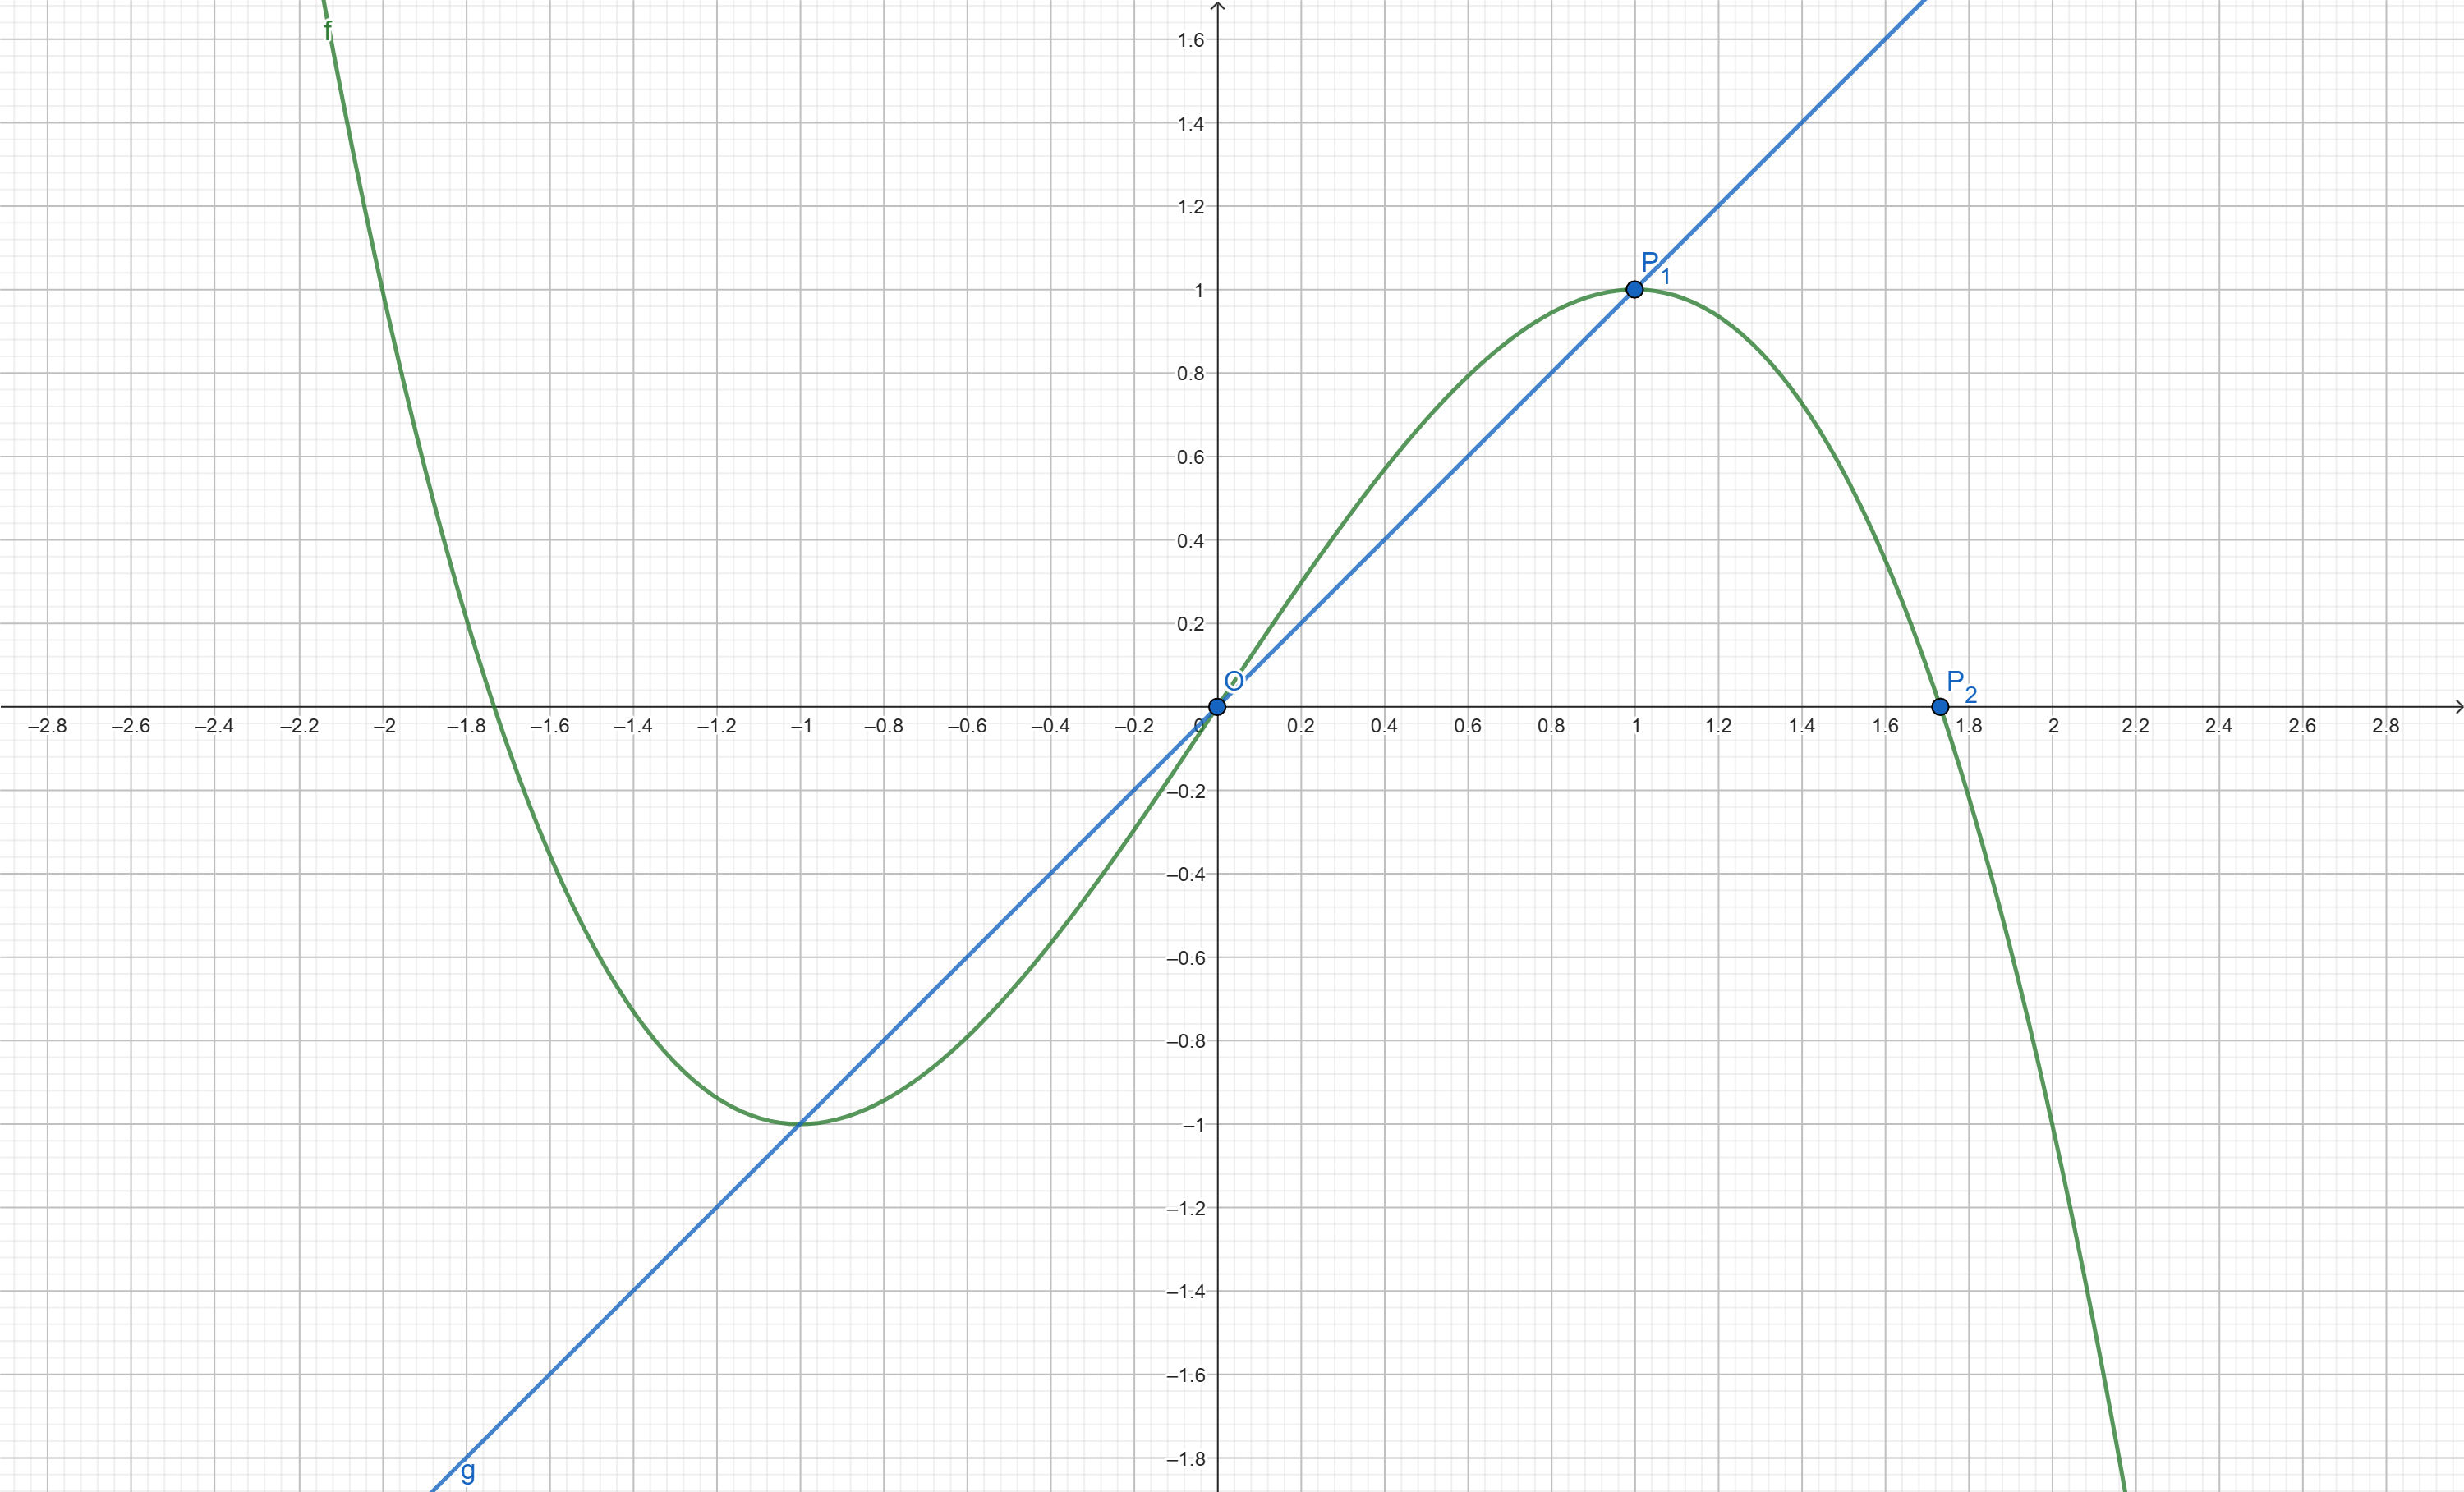
\includegraphics[width=1\linewidth]{schulz-iteration.png}
\caption{\label{fig:Schulz Iteration} The functions $f: y = \frac{1}{2}x(3 - x^2)$ and $g:y=x$ are plotted. Points $O$, $P_1$ and $P_2$ are $(0,0)$, $(1, 1)$ and $(\sqrt{3}, 0)$ respectively.}
\end{figure}
\begin{flushleft}
As is evident from the figure, the map has 3 fixed points, of which $x^*=1$, and $x^*=-1$ are attractive fixed points, and $x^*=0$ is a repelling fixed point. To show this, We can show that $f'(x)$ at $x=1$ and $x=-1$ is $0$, which is less than $1$. For $x=0$, however, it is $\frac{3}{2}$.
\newline
\vspace{1mm}

Between the points $O$ and $P_1$, $f > g$, so, any iteration that enters the region between $0$ and $1$ will end up at $P_1$. Similarly, any iteration that enters the region between $0$ and $-1$ will end up attracted to $-1$. As is evident, initial values up to $P_2$ are guaranteed to enter the region $(0, 1)$ and will be attracted to $x^*=1$. The points immediately beyond $P_2$ will enter a region where they will be attracted to $x*=-1$, followed by a region from which the points are attracted to $x^*=1$ again, till they reach a point where they diverge completely. We can obtain the exact points that mark the complicated basins of attraction of the two fixed points, but it will suffice for this problem to only regard the first region where the points are guaranteed to converge to $x^*=1$. Thus, the largest singular value of $A$ must be less than $\sqrt{3}$. 
\end{flushleft}
\newpage
\section{Part 8}

\begin{flushleft}

Assuming LU Factorization to compute the inverse of the square matrix of size n have an operation count of $\frac{2n^3}{3}$. For Matrix Multiplication, we have an operation count of $2n^3$. But, for the first multiplication of Newton-Schulz, the term inside the bracket $X_k^* X_k$, due to symmetry, would only need half the number of operations. And, the second multiplication, $X_k * (3I - X_k^* X_k)$, would be a regular matrix multiplication with $2n^3$ operations. So, the total operation count for one step of Newton-Schulz is $3n^3$. 
\vspace{1mm}

So, one step of Newton-Schulz takes 4.5 times the number of operations of a step of Newton method.
\vspace{1mm}

Ignoring operation counts, however, in a step of Newton iteration, we have one matrix inversion, while a step of Newton-Schulz has two matrix multiplication steps. So, if matrix multiplication is more than twice as fast as matrix inversion, Newton-Schulz would be a faster operation.

\end{flushleft}

\section{Part 9}
\begin{flushleft}

The condition for convergence of the Newton-Schulz iteration is that the largest singular value of the matrix $X_0$, from which we start the iteration, be smaller than $\sqrt{3}$. This means that the 2-norm of the matrix must be smaller than $\sqrt{3}$. But, it is expensive to calculate the 2-norm of a Matrix, and doing it at every step of the Newton iterations would be very inefficient. One can estimate the 2-norm of a Matrix by using the identity $||A||_2 \leq \sqrt{||A||_1 . ||A||_\infty}$ since calculating $||A||_1$ and $||A||_\infty$ are cheaper operations.

The remarks for running the poldec function, which is written in poldec.m on the given matrices are in the following subsections.

\subsection{rand(10)}
The method took 9 iterations and did not switch to N-S. All of the iterations were Newton-iterations.
\subsection{eye(8)}
The method did not iterate at all since the convergence condition was satisfied with $X_0 = I_8$
\subsection{hilb(6)}
The program took 29 iterations to complete. It switched to N-S iterations from the 23rd iteration.
\subsection{magic(6)}
The program ran 56 iterations but did not converge to a polar decomposition. The reason is that the magic matrices with even size are singular (except for size 2). In the case of magic(6), the rank is 5.
Warning: Matrix is close to singular or badly scaled. Results may be inaccurate. RCOND =  2.000402e-18.
\subsection{hadamard(8)}
The program converged in 6 iterations. Did not switch to N-S iterations.

\end{flushleft}

\newpage
\section{Part 10}

\begin{flushleft}
For a Hermitian positive-definite matrix $A$, the Cholesky decomposition breaks the matrix into factors: $A = L L^*$, where $L$ is a lower triangular matrix (for symmetric positive-definite matrices, $L$ would be real, so $L^* = L'$). Now let $A = L L^*$, and Let $L^*$ have the polar decomposition $L^* = UH$. Then,
\begin{align*}
    LL^* &= (UH)^*.(UH)\\
    &= H^*(U^*U)H\\
    &= H^*H\\
    &= H^2  & [\because H^*=H]
\end{align*}

So, $A =LL^*= H^2$. $H$ is the square root of the matrix $A$.

Code is written in sqrt.m. Note: the function chol in Matlab returns the upper triangular matrix $L^*$ instead of $L$.
\end{flushleft}

\end{document}